\documentclass[../document.tex]{subfiles}

\begin{document}
    \newcommand{\lcfrs}{linear context-free rewriting system}
    \newcommand{\dcp}{definite clause program}
    \chapter{Grammar Formalisms}
    This chapter describes three grammar formalisms that we use for parsing natural language sentences.
    For the subject of this thesis, let us consider a grammar as a collection of rules that are capable of deriving either strings or trees.
    All considered grammar formalisms share the same fundamental structure of their rules:
        Each consists of a sequence of nonterminal symbols, one of which is called the left-hand side (\abrv{lhs}) nonterminal and the rest the right-hand side (\abrv{rhs}) nonterminals, and an expression that computes strings or trees based on an argument for each \abrv{rhs} nonterminal.
        The symbols, that are occurring in these expressions and are part of the result, are called terminal symbols.
    The nonterminals already hint at the recursive structure of grammar derivations: the arguments used to compute the result are computed by successor rules whose \abrv{lhs} nonterminal match the right-hand side nonterminals.

%    However, we will not use grammars to derive any strings, but the opposite:
%        We analyze strings in consideration which collection of grammar rules may be used to derive a given string.
%    This process is called parsing.
%    Usually, the result of this process is not a collection of grammar rules but a digest of it, called derivation tree.

    First, we focus on linear context-free rewriting systems (\abrv{lcfrs}), an extension of context-free grammars introduced by \citet{VijWeiJos87} and extensively studied by \citet{SekMatFujKas91}.
    In this formalism, each rule produces a tuple of strings which may occur in non-consecutive parts in a finally derived string.
    This is used to model sentence positions in the yield of discontinuous constituents.
    When \abrv{lcfrs} are used for parsing of constituency structures, we typically find a rule derivation that computes the input sentence and assume the nonterminals occurring in the derivation as constituency structure.
    \todo{Verwandschaft mit pmcfg, mcfg, tree adjoining grammars, head grammars, minimalist grammars, range concatenation grammars}
    \todo{auch notation range concatenation grammars}

    Secondly, we have a look at a subset of definite clause programs (\abrv{dcp}), which were introduced by \cite{Der85} as a logic characterization of attribute grammars.
    They were used in the context of parsing by \cite{Ned14,Geb17,Geb20} in combination with \abrv{lcfrs} forming hybrid grammars (see next paragraph).
    In contrast to context-free grammars and \abrv{lcfrs}, each rule in this grammar formalism computes a collection of trees instead of strings.
    However, in the scope of this thesis, we consider only \abrv{dcp} rules that produce consecutive parts in trees.
    During parsing with these \abrv{dcp}, we find a derivation with the rules in a grammar that produces a tree with the input sentence as yield and assume the tree as constituency structure.

    The last formalism among the considered are \abrv{lcfrs}/\abrv{dcp} hybrid grammars as introduced by \citet{Ned14}.
    They combine the two aforementioned grammar formalisms:
        Besides the nonterminals, each rule contains the expression of an \abrv{lcfrs} as well as the expression of a \abrv{dcp}.
    During parsing, we find a derivation such that the \abrv{lcfrs} expressions produce the input sentence, the \abrv{dcp} expressions yield the constituency structure.

    In the following sections for each of the three formalisms, the grammars are described gradually:
    \begin{inparaenum}[(i)]
        \item Each section starts with the expressions contained in each rule that compose strings or trees.
        \item After that, they express the rules and the other components in a grammar.
        \item Finally, they explain the derivations in a grammar in tandem with their computed yield and parse\todo{find a name for the string/tree of a derivation}.
    \end{inparaenum}
    Each of these subsections is accompanied by examples that give intuitions for the described structures.

    \section{Linear Context-Free Rewriting Systems}

    In linear context-free rewriting systems (\abrv{lcfrs}), each rule composes a tuple of strings from arguments that are string tuples as well.
    The first definition formalizes the notation for such functions using binary variables that determine an argument (subscript) and one of its components (superscript).
    The sets of compositions are restricted such that the variables occur ordered according to their sub- and superscripts, and no variables for consecutive components of the same argument occur next to each other.
    These restrictions enforce a normal form for \abrv{lcfrs} that matches the properties of grammars extracted from treebanks.
    The normal form itself, however, is not restrictive: For every \abrv{lcfrs}, there is an equivalent \abrv{lcfrs} in normal form. [\citealp[Lem.~2.2]{SekMatFujKas91}; \citealp[Def.~7.2]{Kal10}]

    \begin{definition}[Compositions]\label{def:lcfrs:comp}
        We fix a set of variables \(\X = \big\{ \x_i^j \mid i, j \in \DN_+ \big\}\) and the \(\DN_+^*\)-indexed family of finite subsets \(\X_{s_1\cdots s_k} = \big\{ \x_i^j \mid i \in [k], j \in [s_i] \big\}\) for each \(k \in \DN\), and \(s_1, \ldots, s_k \in \DN_+\).
        Let \(\varSigma\) be a finite set disjoint from \(\X\).
        The family of \abrv{lcfrs} \deflab<\lcfrs>[lcfrs:comp]{composition}[compositions]\todo{define one composition and then the sets of compositions} over \(\varSigma\), denoted by \(\C^\varSigma\), is the \(\DN_+^+\)-indexed family over sets of non-empty sequences over strings in \((\varSigma \cup \X)^+\) such that for each \(k \in \DN\) and \(s_1, \ldots, s_k, s \in \DN_+\), the set \(\C^\varSigma_{s_1 \cdots s_k s}\) contains each sequence \(u_1, \ldots, u_s \in (\varSigma \cup \X_{s_1 \cdots s_k})^+\) of length \(s\) such that
        \begin{compactenum}[(i)]
            \item each variable in \(\X_{s_1 \cdots s_k}\) occurs exactly once in the string \(u_1 \cdots u_s\),
            \item for each \(i \in [k-1]\), the variable \(\x_i^1\) occurs to the left of \(\x_{i+1}^1\) in the string \(u_1 \cdots u_s\),
            \item for each \(i \in [k]\) and \(j \in [s_i-1]\), the variable \(\x_i^j\) occurs to the left of \(\x_i^{j+1}\) in the string \(u_1 \cdots u_s\),
            \item there are no \(i \in [k]\) and \(j \in [s_i-1]\) such that \(\x^j_i\x^{j+1}_i\) is a subsequence in any of \(u_1, \ldots, u_s\).
        \end{compactenum}
        We associate the identifier \(\C^\varSigma\) with the set of all \abrv{lcfrs} compositions \[
            \bigcup_{k \in \DN, s_1, \ldots, s_k, s \in \DN_+} \C^{\varSigma}_{s_1 \cdots s_k s} \text{.}
        \]

        We associate a function, denoted by \(\sem{(u_1, \ldots, u_s)}\), from \(k\) string tuples, where the \(i\)-th tuple is of length \(s_i\), to a string tuple of length \(s\) with each composition in \((u_1, \ldots, u_s) \in \C^\varSigma_{(s_1\cdots s_k s)}\).
        Given the arguments \(\big(v_i = (v_i^j \mid j \in [s_i]) \mid i \in [k]\big)\), the result is the string tuple \(
            \sem{(u_1, \ldots, u_s)}(v_1, \ldots, v_k) = (u_1[\phi], \ldots, u_s[\phi])
        \) where \(\phi\) is the \(\X_{s_1 \cdots s_k}\)-indexed family with \(\phi_{x_i^j} = v_i^j\).
        Intuitively, this function replaces each occurring variable of the form \(\x_i^j\) in \(u_1, \ldots, u_s\) with the \(j\)-th component of the \(i\)-th argument.
    \end{definition}

    \begin{example}\label{ex:lcfrs:comp}
       Consider an alphabet \(\Sigma=\{\tn{A}, \tn{hearing}, \tn{is}, \tn{scheduled}, \tn{on}, \tn{the}, \tn{issue}, \tn{today}\}\) and the following compositions:
        \begin{align*}
            c_1 &= (\tn{A}), & c_2 &= (\tn{today}), & c_3 &= (\tn{issue}) && \in \C^\Sigma_{(1)} \\
            c_4 &= (\tn{the} \, \x_1^1), & c_5 &= (\x_1^1 \, \tn{hearing}) & & && \in \C^\Sigma_{(1\,1)} \\
            c_6 &= (\x_1^1 \, \tn{is} \, \x_1^2) && && && \in \C^\Sigma_{(2\,1)} \\
            c_7 &= (\x_1^1, \tn{on} \, \x_2^1) && && && \in \C^\Sigma_{(1\,1\,2)}   \\
            c_8 &= (\x_1^1, \tn{scheduled} \, \x_1^2 \, \x_2^1) && && && \in \C^\Sigma_{(2\,1\,2)}
        \end{align*}

        The subscript indexing the family of compositions \(\C^\Sigma\) determines the arity of the associated functions.
        E.g.\@ \(\sem{c_1} \in \C^\Sigma_{(1)}\) takes no arguments (it is constant) and yields a single string,
            \(\sem{c_8} \in \C^\Sigma_{(2\,1\,2)}\) takes two arguments, a sequence over strings of length 2 and 1, and gives a sequence of length 2 as a result.
        For example:
        \begin{multline*}
            \sem{c_8}\Big( \; \big( \tn{A hearing}, \: \tn{on the issue} \big), \, \big( \tn{today} \big) \; \Big)
            \\= \big( \tn{A hearing}, \: \tn{scheduled on the issue today} \big)
        \end{multline*}

        The functions may form terms, e.g.
        \begin{align*}
            \sem{c_7}\Big( \; \sem{c_5}\big(\,\sem{c_1}()\,\big), \: \sem{c_4}\big(\,\sem{c_3}()\,\big) \; \Big)
                =& \sem{c_7}\Big( \; \sem{c_5}\big(\tn{A}\big), \: \sem{c_4}\big(\tn{issue}\big) \; \Big) \\
                =& \sem{c_7}\Big( \; (\tn{A hearing}), \: (\tn{the issue}) \; \Big) \\
                =& (\tn{A hearing}, \: \tn{on the issue})
        \end{align*}
    \end{example}

    \begin{definition}[\abrv{Lcfrs} Grammar]
        A \deflab[lcfrs]{\lcfrs} (\abrv{lcfrs})%
        \defabrv{\lcfrs}{\abrv{lcfrs}}
        is a tuple \(G=(N, \varSigma, S, R)\) where
        \begin{compactenum}[(i)]
            \item \(N\) is a finite set (\emph{nonterminals}),
            \item \(\varSigma\) is an alphabet (\emph{terminals}),
            \item \(S \in N\) (initial non-terminal),
            \item \(R\) is a finite subset of \(N \times \C^\varSigma \times N^*\) (\emph{rule}),\todo{define set of rules over \(N, \varSigma\) and families} and
            \item there is an implicit positive integer \(\fanout(A) \in \DN_+\), called the \deflab<\lcfrs>[lcfrs:fo]{fanout} for each nonterminal \(A \in N\), such that
            for each \((A, c, B_1\cdots B_k) \in R\), the \abrv{lcfrs} composition \(c\) is an element of \(\C^\varSigma_{\fanout(B_1) \cdots \fanout(B_k) \fanout(A)}\).
        \end{compactenum}

        Rules are denoted in the form \(A \to c\,(B_1, \ldots, B_k)\) instead of \((A, c, B_1 \cdots B_k)\); \(A\) is called the left-hand side (\abrv{lhs}) nonterminal and \(B_1, \ldots B_k\) are the right-hand side (\abrv{rhs}) nonterminals, \(c\) is the composition of the rule.
        The natural \(k\) is the \deflab<\lcfrs>[lcfrs:rk]{rank} of the rule; the \emph{rank of the grammar \(G\)} is the maximum rank occurring in the rules of \(G\).
    \end{definition}

    \begin{definition}[Grammar forms]
        We distinguish rules and grammars of the following form:
        \begin{compactitem}
            \item Rules of rank zero, one and two are called \emph{nullary}, \emph{unary} and \emph{binary}, respectively.
            \item Lcfrs containing only nullary, unary and binary rules are called \deflab<\lcfrs>[lcfrs:bin]{binary}.
            \item Rules whose composition contains exactly one terminal in \(\varSigma\) are called \deflab<\lcfrs>[lcfrs:lex]{lexical}.
            \item Lcfrs containing only lexical rules are called \emph{lexical}.
            \item Rules whose composition contain no terminal at all are called \emph{non-lexical}.
            \item Lcfrs that contain only lexical nullary rules and non-lexical rules of rank \(\ge 1\) are called \deflab<\lcfrs>[lcfrs:simple]{simple}.
        \end{compactitem}
    \end{definition}

    \begin{example}[Continues \cref{ex:lcfrs:comp}]\label{ex:lcfrs:rules}
        Consider the alphabet \(\mathrm{N} = \{\nt{vp}, \nt{vp}_2, \nt{np}, \nt{np}_2, \nt{pp}, \nt{np}^\nt{L}\}\) of nonterminal symbols and the \abrv{lcfrs} \(\mathrm{G} = (\mathrm{N}, \Sigma, \nt{vp}, \mathrm{R})\) with
        \begin{align*}
            \mathrm{R} = \big\{\;
                \nt{n}^\nt{l} &\to (\tn{A})\:(), &\nt{n} &\to (\tn{issue})\:(), &\nt{n} &\to (\tn{today})\:(), &\\
                \nt{n} &\to (\x_1^1 \, \tn{hearing})\:(\nt{n}^\nt{l}), &\nt{p} &\to (\tn{the}\,\x_1^1)\:(\nt{n}), \\
                \nt{n}_2 &\to (\x_1^1, \tn{on} \, \x_2^1)\:(\nt{n}, \nt{p}), \\
                \nt{v}_2 &\to (\x_1^1, \tn{scheduled} \, \x_1^2 \, \x_2^1)\:(\nt{n}_2, \nt{n}), \\
                \nt{v} &\to (\x_1^1 \, \tn{is} \, \x_1^2)\:(\nt{v}_2)
            &&&&&\;\big\}
        \end{align*}
        The fanout for each nonterminal \(A\) determines the length of the composition with \abrv{lhs} \(A\) and the number of variables if \(A\) occurs in the \abrv{rhs} nonterminals of a rule.
        In the above example, the nonterminal symbols with subscript \(_2\), i.e.\@ \(\nt{n}_2\) and \(\nt{v}_2\), are of fanout 2, and all others of fanout 1.
        The composition of the rule \(\nt{v}_2 \to (\x_1^1, \tn{scheduled} \, \x_1^2 \, \x_2^1)\:(\nt{n}_2, \nt{n})\) is of length \(\fanout(\nt{v}_2) = 2\) and there are \(\fanout(\nt{n}_2) = 2\) variables for the first \abrv{rhs} nonterminal and \(\fanout(\nt{n}) = 1\) for the second.
        \todo{G is lexical, example for simple lcfrs?}
    \end{example}

    \begin{definition}[Derivation]
        Let us consider an lcfrs \(G = (N, \varSigma, S, R)\).
        An \abrv{lcfrs} \deflab<\lcfrs>[lcfrs:deriv]{derivation} is a tree over rules in \(\T_R\) that suffices the following conditions:
        \begin{compactitem}
            \item Each leaf is equipped with a nullary rule as symbol.
            \item Each inner node is a rule with the same amount of \abrv{rhs} nonterminals as children in the tree such that the \(i\)-th \abrv{rhs} nonterminal is the \(i\)th child's \abrv{lhs} nonterminal.
        \end{compactitem}
        The set of all \abrv{lcfrs} derivations is denoted by \(\derivs^R\).
        We identify this set with the \(N\)-indexed partition of \(\derivs^R\) that assigns each nonterminal \(A\) to the derivations whose root is equipped with \abrv{lhs} \(A\).
    \end{definition}

    \begin{definition}[Yield and Parse]
        Consider a derivation \(d\) in \(\derivs^R_A\) of the form \(d = r\,(d_1, \ldots, d_k)\) where the root \(r\) is of the form \(A \to c\,(B_1, \ldots, B_k)\).
        The \deflab<\lcfrs>[lcfrs:yd]{yield} of \(d\) is defined recursively: \(\yield(d) = \sem{c}(\yield(d_1), \ldots, \yield(d_k))\).
        For the definition of the parse of \(d\), let us consider the sequences of terminal symbols \(w_1, \ldots, w_{k+1} \in \varSigma^*\) such that,
        \begin{compactitem}
            \item \(w_1\) is the sequence of terminal symbols occurring before the variable \(\x_1^1\) in \(c\),
            \item for each \(i \in \{2, \ldots, k\}\), \(w_i\) is the sequence of terminal symbols occurring between the variables \(\x_{i-1}^1\) and \(\x_i^1\) in \(c\), and
            \item \(w_{k+1}\) is the sequence of terminal symbols occurring after the variable \(\x_k^1\) in \(c\).
        \end{compactitem}
        Then the \deflab<\lcfrs>[lcfrs:parse]{parse} of \(d\) is the tree \[
            \parse(d) = A(w_1, \parse(d_1), w_2, \parse(d_2), \ldots, w_k, \parse(d_k), w_{k+1}) \text{.}
        \]
    \end{definition}

    \begin{example}[Continues \cref{ex:lcfrs:comp,ex:lcfrs:rules}]\label{ex:lcfrs:deriv}
        Let's consider the two trees illustrated below, the left one \(d\) is a tree over rules in the \abrv{lcfrs} \(\mathrm{G} = (N, \Sigma, \nt{v}, R)\), the right one is an element in \(\T_N(\Sigma)\).
        Its root has the \abrv{lhs} \(\nt{n}_2\), the tree is an element of \(\derivs^R_{\nt{n}_2}\).
        The yield of \(d\) is term over compositions computed in \cref{ex:lcfrs:comp}: \(\yield(d) = (\tn{A hearing}, \: \tn{on the issue})\).
        The parse of \(d\) is illustrated to the right of \(d\).

        \null\hfill
        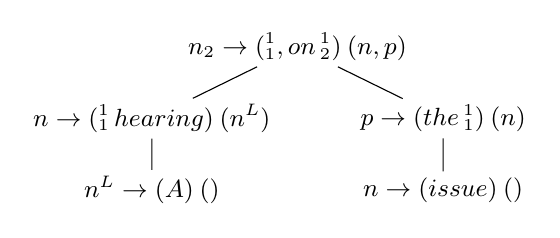
\begin{tikzpicture}[level distance=6ex, font=\small, sibling distance=3.7cm, inner sep=2pt]
            \node {\(\nt{n}_2 \to (\x_1^1, \tn{on} \, \x_2^1)\:(\nt{n}, \nt{p})\)}
            child {node {\(\nt{n} \to (\x_1^1 \, \tn{hearing})\:(\nt{n}^\nt{L})\)}
                child {node {\(\nt{n}^\nt{L} \to (\tn{A})\:()\)}}}
            child {node {\(\nt{p} \to (\tn{the}\,\x_1^1)\:(\nt{n})\)}
                child {node {\(\nt{n} \to (\tn{issue})\:()\)}}};
        \end{tikzpicture}
        \hfill
        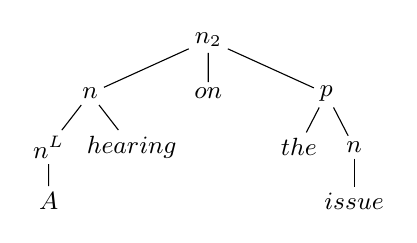
\begin{tikzpicture}[level distance=4.5ex, font=\small, inner sep=2pt]
            \node {\(\nt{n}_2\)}
            child {node {\(\nt{n}\)}
                [sibling distance=3em]
                child {node {\(\nt{n}^\nt{L}\)}
                    child { node {\(\tn{A}\)}}}
                child {node {\(\tn{hearing}\)}}}
            child {node {\(\tn{on}\)}}
            child {node {\(\nt{p}\)}
                [sibling distance=2em]
                child {node {\(\tn{the}\)}}
                child {node {\(\nt{n}\)}
                    child { node {\(\tn{issue}\)}}}};
        \end{tikzpicture}
        \hfill\null
    \end{example}


    \section{Definite Clause Programs (\abrv{dcp})}
    \abrv{dcp}{}s are, in contrast to \abrv{lcfrs}, a formalism where each rule produces trees instead of plain strings.
    The most striking difference to the previous formalism, however, lies in the composition expressions contained in each rule:
        They do not only allow substitution with parameters produced by successors in a derivation (first order substitution), but each single parameter may also contain variables that are substituted in the same step (second order substitution).
    This corresponds to the information flow from bottom to the top in a derivation as expressed by synthetic attributes (first order substitution), as well as the information flow from top to the bottom in a derivation by inherent attributes (second order substitution) in attribute grammars.
    The implementation of these two systems of substitution, two pairwise distinct sets of variables are used: \(\X\) for the first (as in \abrv{lcfrs}), and \(\Y\) for the second order substitution.

    In their most general form, the object produced by a derivation in such a \abrv{dcp} is not necessarily computable, as the two types of substitution may mutually recur.
    To solve this issue, there were some restrictive forms introduced which exclude circular dependencies in the expressed productions. \citep[Sec.~3.4 about non-circular attribute grammars]{Cou82}
    It is easy to see that the definition shown in this section supersedes each of these restricted forms, as it exclusively allows fixed terminal objects or a single second order variable as parameter for second order substitution.
    To avoid unnecessarily complicated definitions, the subset of \abrv{dcp} shown in this section is even further restricted such that
    \begin{inparaenum}
        \item it deals with ranges\todo{def. range} of consecutive subtrees (and not sequences of ranges), and
        \item each rule's composition expression allows exactly one second-order substitution (which may be the empty sequence).
    \end{inparaenum}

    \begin{definition}[Composition]
        We fix the \(\DN\)-family of finite sets of variables \((\X_k = \{\x_i \mid i \in [k]\} \mid k \in \DN)\), and the singleton set \(\Y = \{\y\}\).
        The identifier \(\X\) denotes the union \(\bigcup_{k \in \DN} \X_k = \{\x_i \mid i \in \DN\}\).
        Let \(\varSigma\) and \(\varGamma\) be alphabets disjoint from \(\X \cup \Y\).
        The \(\DN\)-family \((S_k = \{x(y) \mid x \in \X_k, y \in \T_\varGamma(\varSigma \cup Y)^*\} \mid k \in \DN)\) denotes expressions for occurrences of first-order substitutions using \(k\) variables.
        The \(\DN\)-family of \abrv{dcp} \deflab<\dcp>[dcp:comp]{composition}[compositions] over \(\varSigma\) and \(\varGamma\) is \((\C^{\varGamma\varSigma}_k \mid k \in \DN)\) such that \(\C^{\varGamma\varSigma}_k\) contains each nonempty sequence \(c\) in \((\T_\varGamma(\varSigma \cup \Y \cup S_k))^+\) such that each variable in \(\X_k \cup \Y\) occurs exactly once in \(c\).
        We associate the identifier \(\C^{\varGamma\varSigma}\) with the set of all such \abrv{dcp} compositions \(\bigcup_{k \in \DN} \C^{\varGamma\varSigma}_{k}\).

        Each composition \(c \in \C^{\varGamma\varSigma}_k\) is associated with a function \[
            \sem{c}\colon \big(\T_\varGamma(\varSigma \cup Y)^*\big)^k \to \T_\varGamma(\varSigma \cup Y)^*
        \] such that \(\sem{c}(\xi_1, \ldots, \xi_k) = c[\x_1=\xi_1, \ldots, \x_k=\xi_k]\) is the second-order substitution of \(\X_k\) in \(c\).
    \end{definition}

%    The occurrences of variables are abbreviated in the following two ways:
%    \begin{compactenum}
%        \item Variables in \(\X\) with successor \(\varepsilon\) are abbreviated by omitting the parentheses and the successor as a whole; e.g.\@ instead of \(\x_1(\varepsilon)\), we just write \(\x_1\).
%        \item We omit trailing occurrences of the variable \(\y\), if it does not occur as a successor of any node; e.g.\@ instead of \(\text{S}(\x_1)\,\y \), we just write \(\text{S}(\x_1)\).
%    \end{compactenum}

    \begin{example}\label{ex:dcp:comp}
        Consider the following compositions over the alphabets \(\varSigma = \{ \cn{sbar}, \cn{s}, \cn{vp}, \cn{np} \}\) and \(\varGamma = \{\tn{where}, \tn{the}, \tn{survey}, \tn{was}, \tn{carried}, \tn{out}\}\):
        \begin{align*}
             c_1 &= \tn{where} \, \y,
            &c_2 &= \y \, \tn{out},
            &c_3 &= \cn{np} (\y \, \tn{survey}) && \in \C_0\\
             c_4 &= \cn{vp}(\x_1(\y) \, \tn{was}) && && && \in \C_1 \\
             c_5 &= \cn{sbar} (\cn{s} (\x_1(\y) \, \x_2(\tn{the}))),
            &c_6 &= \cn{vp}(\x_1(\y) \, \x_2(\tn{carried})) && && \in \C_2
        \end{align*}
        The subscript indexing the family of compositions \(\C\) determines the number of arguments for the functions represented by the elements in \(\C\).
        E.g.\@ \(\sem{c_1}\) takes no arguments, and \(\sem{c_6}\) takes two arguments.
        Evaluating any term of such compositions yields a sequence tree in \(\T_\varSigma(\varGamma \cup \Y)\) with exactly one occurrence of \(\y\), for example:
        \begin{align*}
            \sem{c_6} \big( \sem{c_1}(), \sem{c_2}() \big)
                &= \sem{c_6} \big( \: (\tn{where} \, \y), \: (\y \, \tn{out}) \: \big) \\
                &= \cn{vp}(\x_1(\y) \, \x_2(\tn{carried}))[\x_1=(\tn{where} \, \y), \x_2=(\y \, \tn{out})] \\
                &= \cn{vp}(\x_1 \, \x_2)[\x_1=(\tn{where} \, \y)[\y=\y], \x_2=(\y \, \tn{out})[\y=\tn{carried}]] \\
                &= \cn{vp}(\x_1 \, \x_2)[\x_1=(\tn{where} \, \y), \x_2=(\tn{carried out})] \\
                &= \cn{vp}(\tn{where} \, \y \, \tn{carried out})
        \end{align*}
    \end{example}

    \begin{definition}[\abrv{dcp} grammar]
        A \deflab[dcp]{definite clause program}%
        \defabrv{\dcp}{\abrv{dcp}}
        is a tuple \(G=(N, \varSigma, S, R)\) where
        \begin{compactenum}[(i)]
            \item \(N\) is a finite set (\emph{nonterminals}),
            \item \(\varSigma\) is an alphabet (\emph{terminals}),
            \item \(S \in N\) (\emph{initial non-terminal}),
            \item \(R\) is a finite subset of \(\bigcup_{k \in \DN} N \times \C^\varSigma_k \times N^k\) such that for each rule \((A, c, B_1\cdots B_k)\) holds: if \(A = S\) then \(c\) is of length 1.
        \end{compactenum}

        Rules are denoted in the form \(A \to c\,(B_1, \ldots, B_k)\) instead of \((A, c, B_1 \cdots B_k)\); \(A\) is called the \abrv{lhs} and \(B_1, \ldots B_k\) are the \abrv{rhs}, \(c\) is the composition of the rule.
        The natural \(k\) is the \emph{rank} of the rule; the rank of the grammar \(G\) is the maximum rank occurring in the rules of \(G\).
    \end{definition}

    \todo{grammar forms: at least lexical}

    We use the same definition for derivations for \abrv{dcp} as for \abrv{lcfrs}.
    However, the terms yield and parse differ, since the grammar produces trees instead of strings.
    We cannot easily enforce that compositions for a start nonterminal produce a single tree.
    Therefore, the definition introduces a fresh symbol \(\cn{root}\) that governs the sequence of trees produced by the compositions of a derivation.

    \begin{definition}[Yield and Parse]
        Consider a derivation \(d\) in \(\derivs^R_A\) of the form \(d = r\,(d_1, \ldots, d_k)\) where the root \(r\) is of the form \(A \to c\,(B_1, \ldots, B_k)\).
        We fix a symbol \(\cn{root}\) that is not in \(\varGamma \cup \varSigma\) and define the \deflab<\dcp>[dcp:parse]{parse} of \(d\) as the tree \[
            \parse(d) = \cn{root}\Big( \sem{c}(\parse(d_1),\ldots,\parse(d_k))[\y=\varepsilon]\Big) \text{.}
        \]
        The \deflab<\dcp>[dcp:yd]{yield} of \(d\) is \(\yield(d) = \yield(\parse(d))\).
    \end{definition}

    \begin{example}[Continues \cref{ex:dcp:comp}]
        Consider the alphabet \(N = \{\nt{v}^\nt{L}, \nt{v}, \nt{n}, \nt{s} \}\) and the \abrv{dcp} \(G = (N, \varSigma, \nt{s}, R)\) where
        \begin{align*}
            R = \Big\{ \quad
            \nt{v}^\nt{L} &\to (\tn{where} \, \y)\:(),
            \quad \nt{v} \to (\y \, \tn{out})\:(),
            &\nt{n} &\to (\cn{np} (\y \, \tn{survey}))\:(), \\
            \nt{v} &\to (\cn{vp}(\x_1(\y) \, \tn{was}))\:(\nt{v}),  \\
            \nt{s} &\to (\cn{sbar} (\cn{s} (\x_1(\y) \, \x_2(\tn{the}))))\:(\nt{v}, \nt{n}),
            &\nt{v} &\to (\cn{vp}(\x_1(\y) \, \x_2(\tn{carried})))\:(\nt{v}^\nt{L}, \nt{v})
            \quad \Big\} \text{.}
        \end{align*}

        The tree \(d\) illustrated below (left) is a derivation in \(\derivs^R_\nt{v}\), its parse is shown to the right of \(d\).
        A part of the computations (for the bottom \(\cn{vp}\)-node) was already shown in the previous example in detail.
        We can read the yield of \(d\) from the leave of the parse: \(\tn{where carried out was}\).

        \null\hfill
        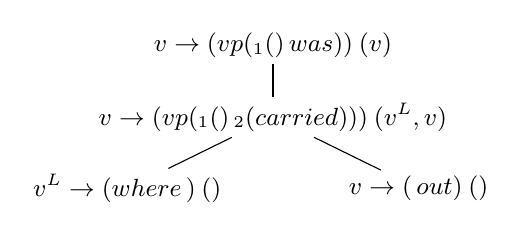
\begin{tikzpicture}[level distance=6ex, font=\small, sibling distance=3.7cm, inner sep=2pt]
            \node {\(\nt{v} \to (\cn{vp}(\x_1(\y) \, \tn{was}))\:(\nt{v})\)}
            child {node {\(\nt{v} \to (\cn{vp}(\x_1(\y) \, \x_2(\tn{carried})))\:(\nt{v}^\nt{L}, \nt{v})\)}
                child {node {\(\nt{v}^\nt{L} \to (\tn{where} \, \y)\:()\)}}
                child {node {\(\nt{v} \to (\y \, \tn{out})\:()\)}}};
        \end{tikzpicture}
        \hfill
        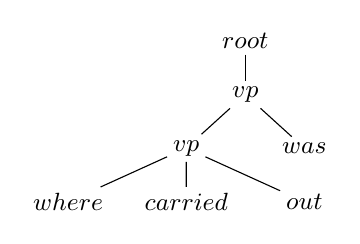
\begin{tikzpicture}[level distance=4.5ex, font=\small, inner sep=2pt]
            \node {\(\cn{root}\)}
            child{ node {\(\cn{vp}\)}
                child {node {\(\cn{vp}\)}
                    child {node {\(\tn{where}\)}}
                    child {node {\(\tn{carried}\)}}
                    child {node {\(\tn{out}\)}}}
                child {node {\(\tn{was}\)}}};
        \end{tikzpicture}
        \hfill\null
    \end{example}

    \section{Hybrid Grammars}

    \ifSubfilesClassLoaded{%
        \printindex
        \bibliography{../references}%
    }{}
\end{document}
